% !TEX root = ../Oliveras_Talk.tex

\section{Implementation}
% ==============================================================================================
\frame[t]{
	\frametitle{Experimental Set-Up}
	\vfill
	\begin{center}
		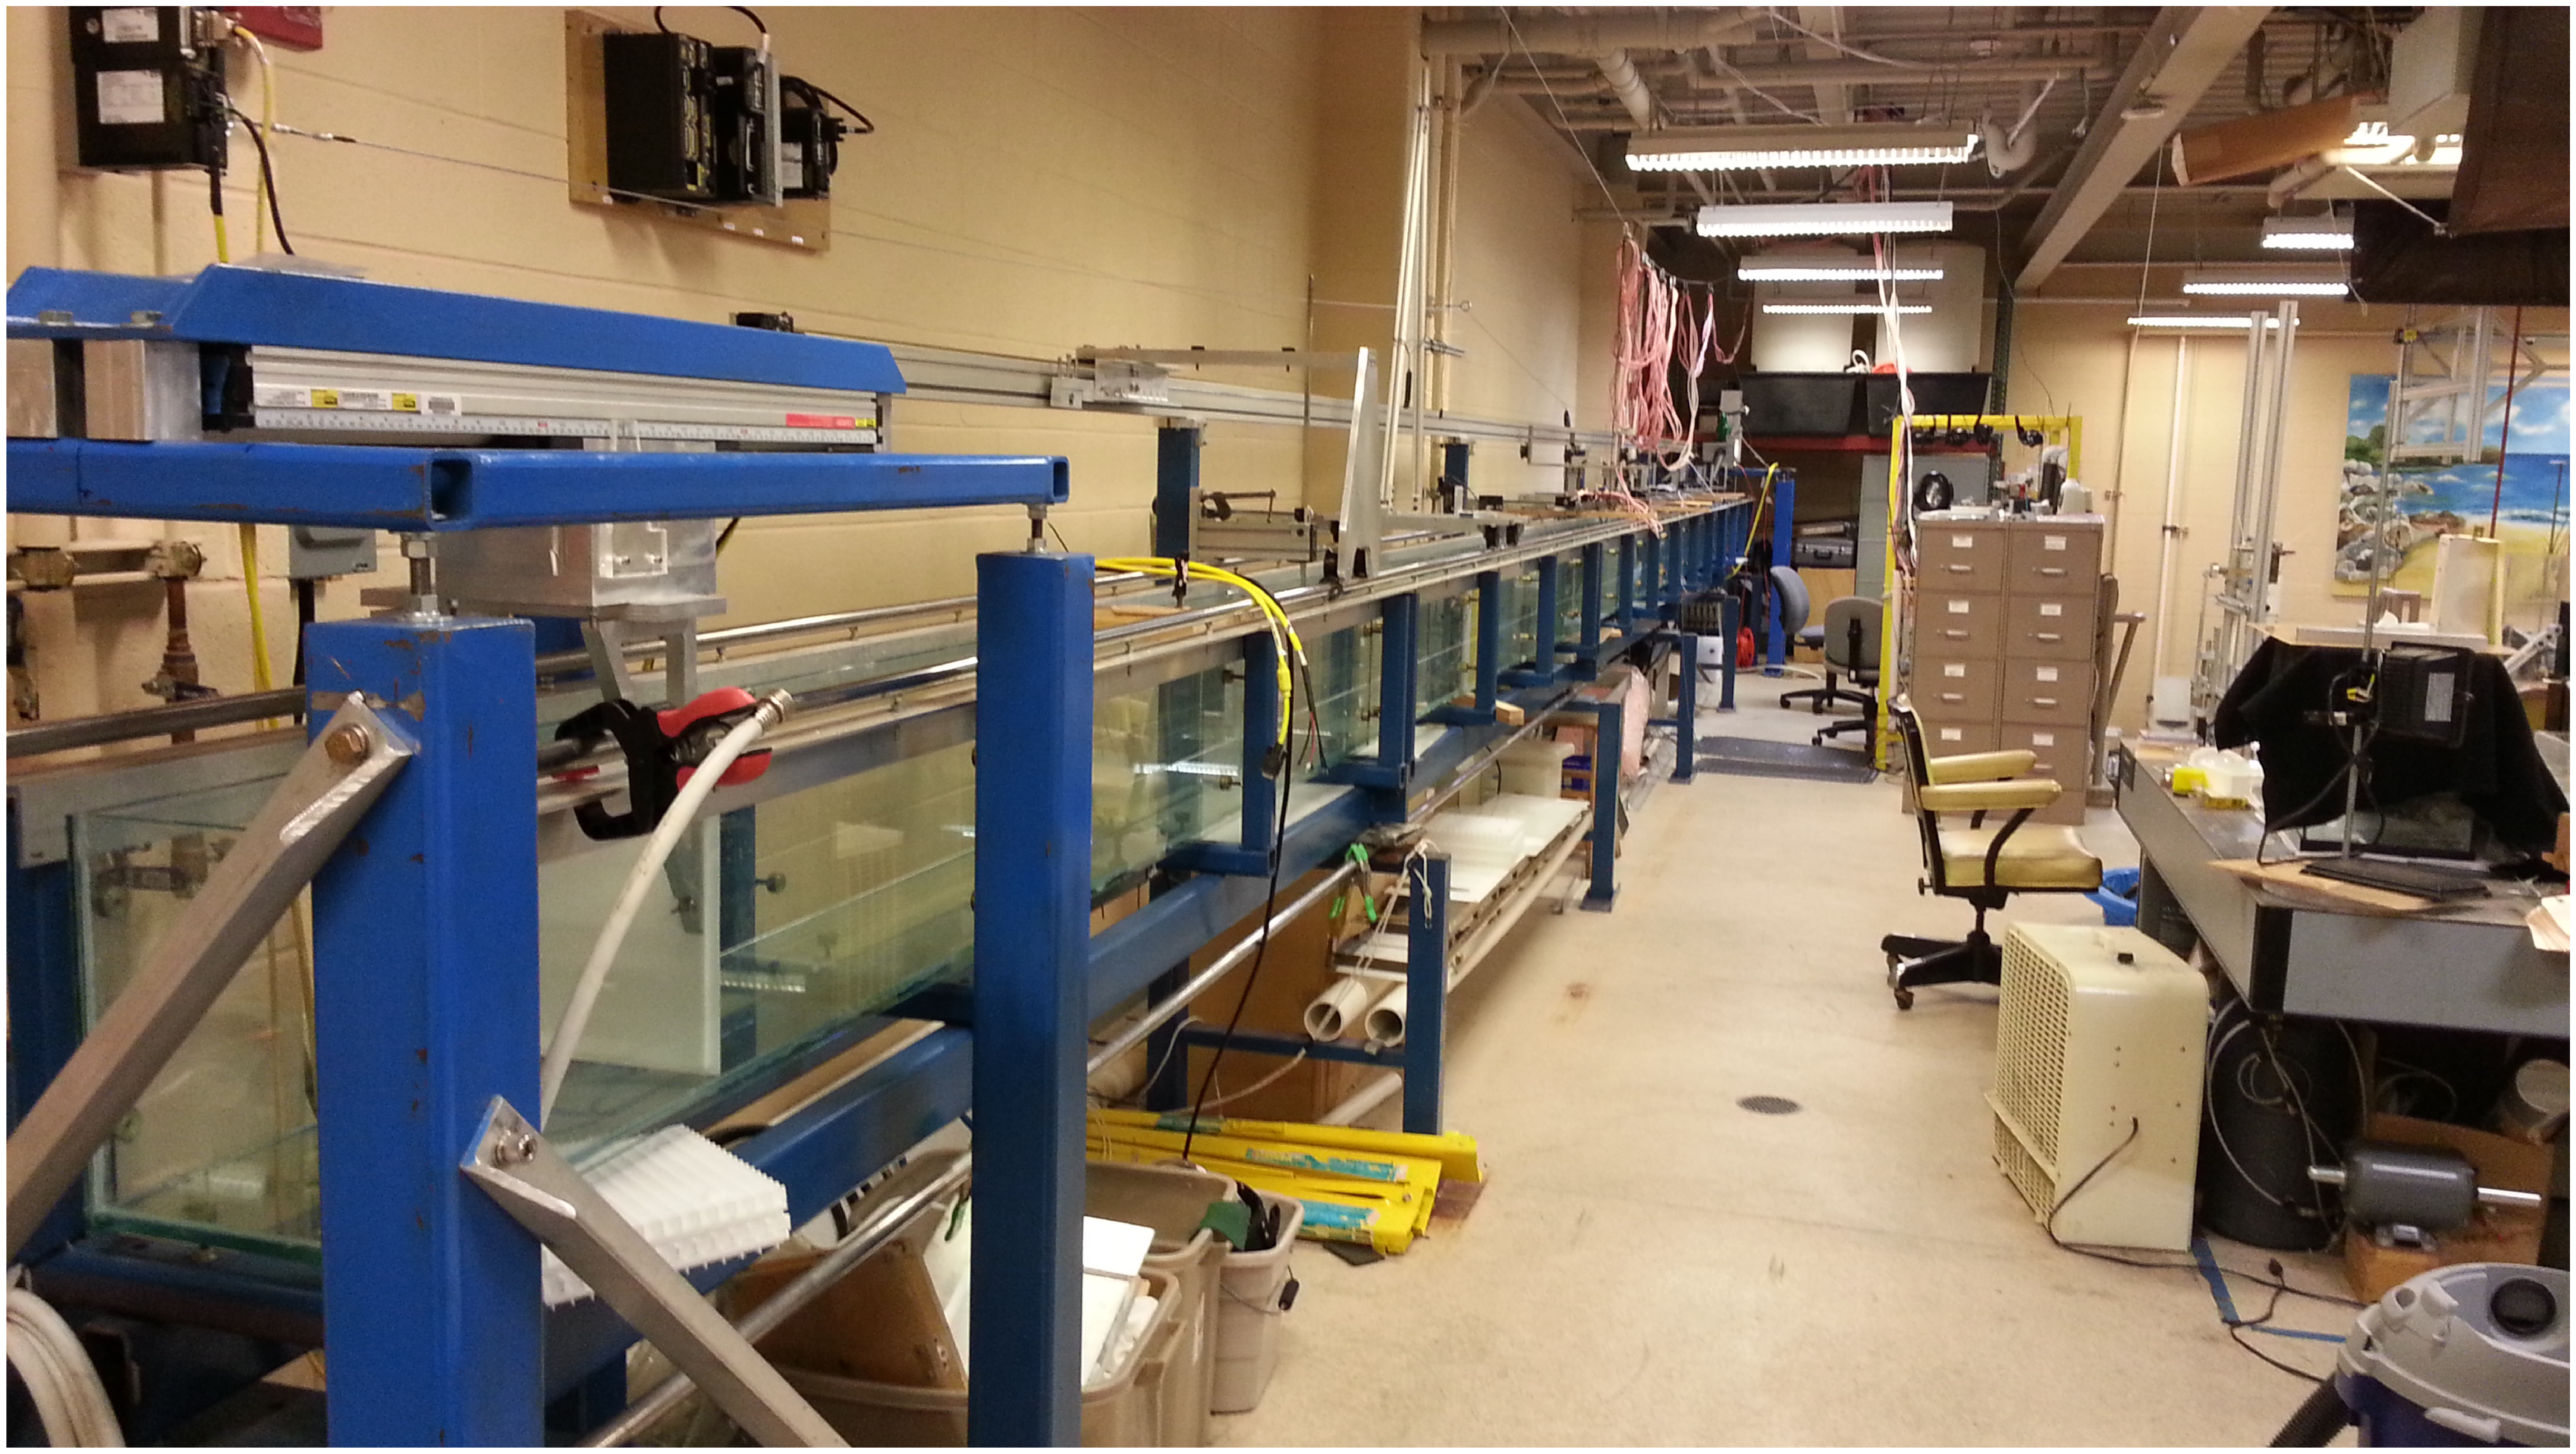
\includegraphics[height=.4\textheight]{images/Tank}
		\vfill
		\vfill
		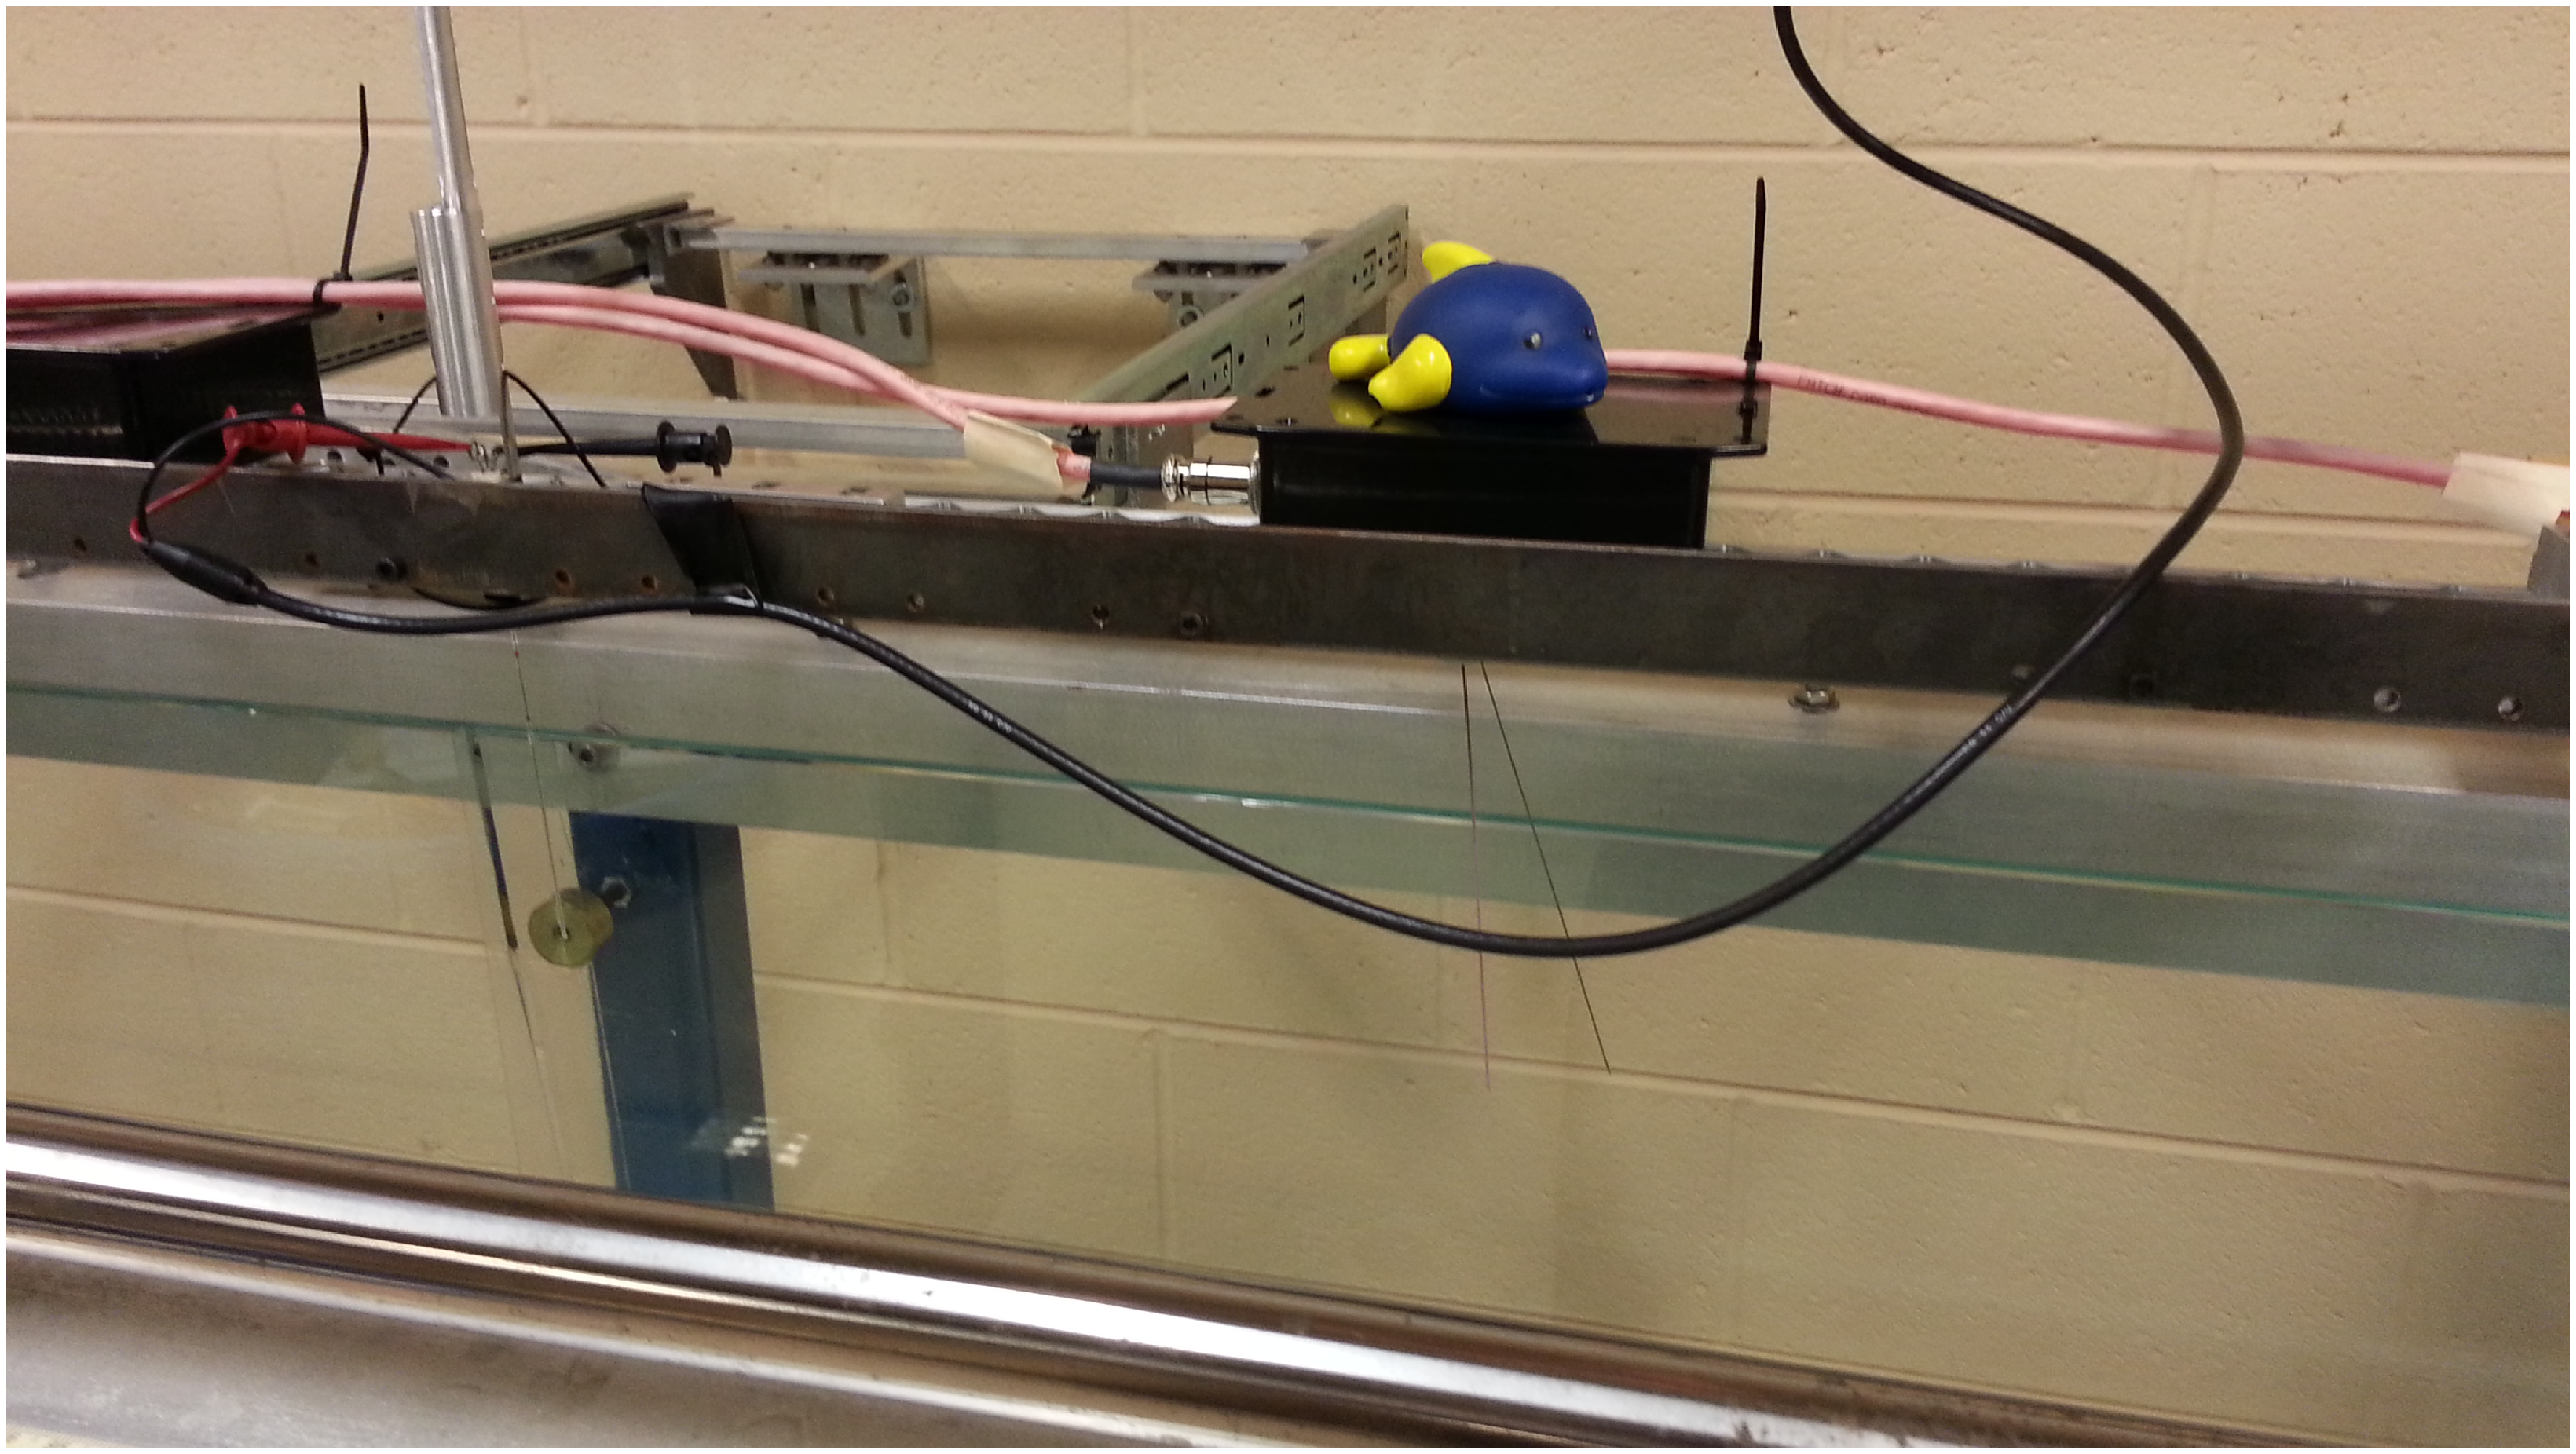
\includegraphics[height=.3\textheight]{images/Surface_Gauge}\hfill 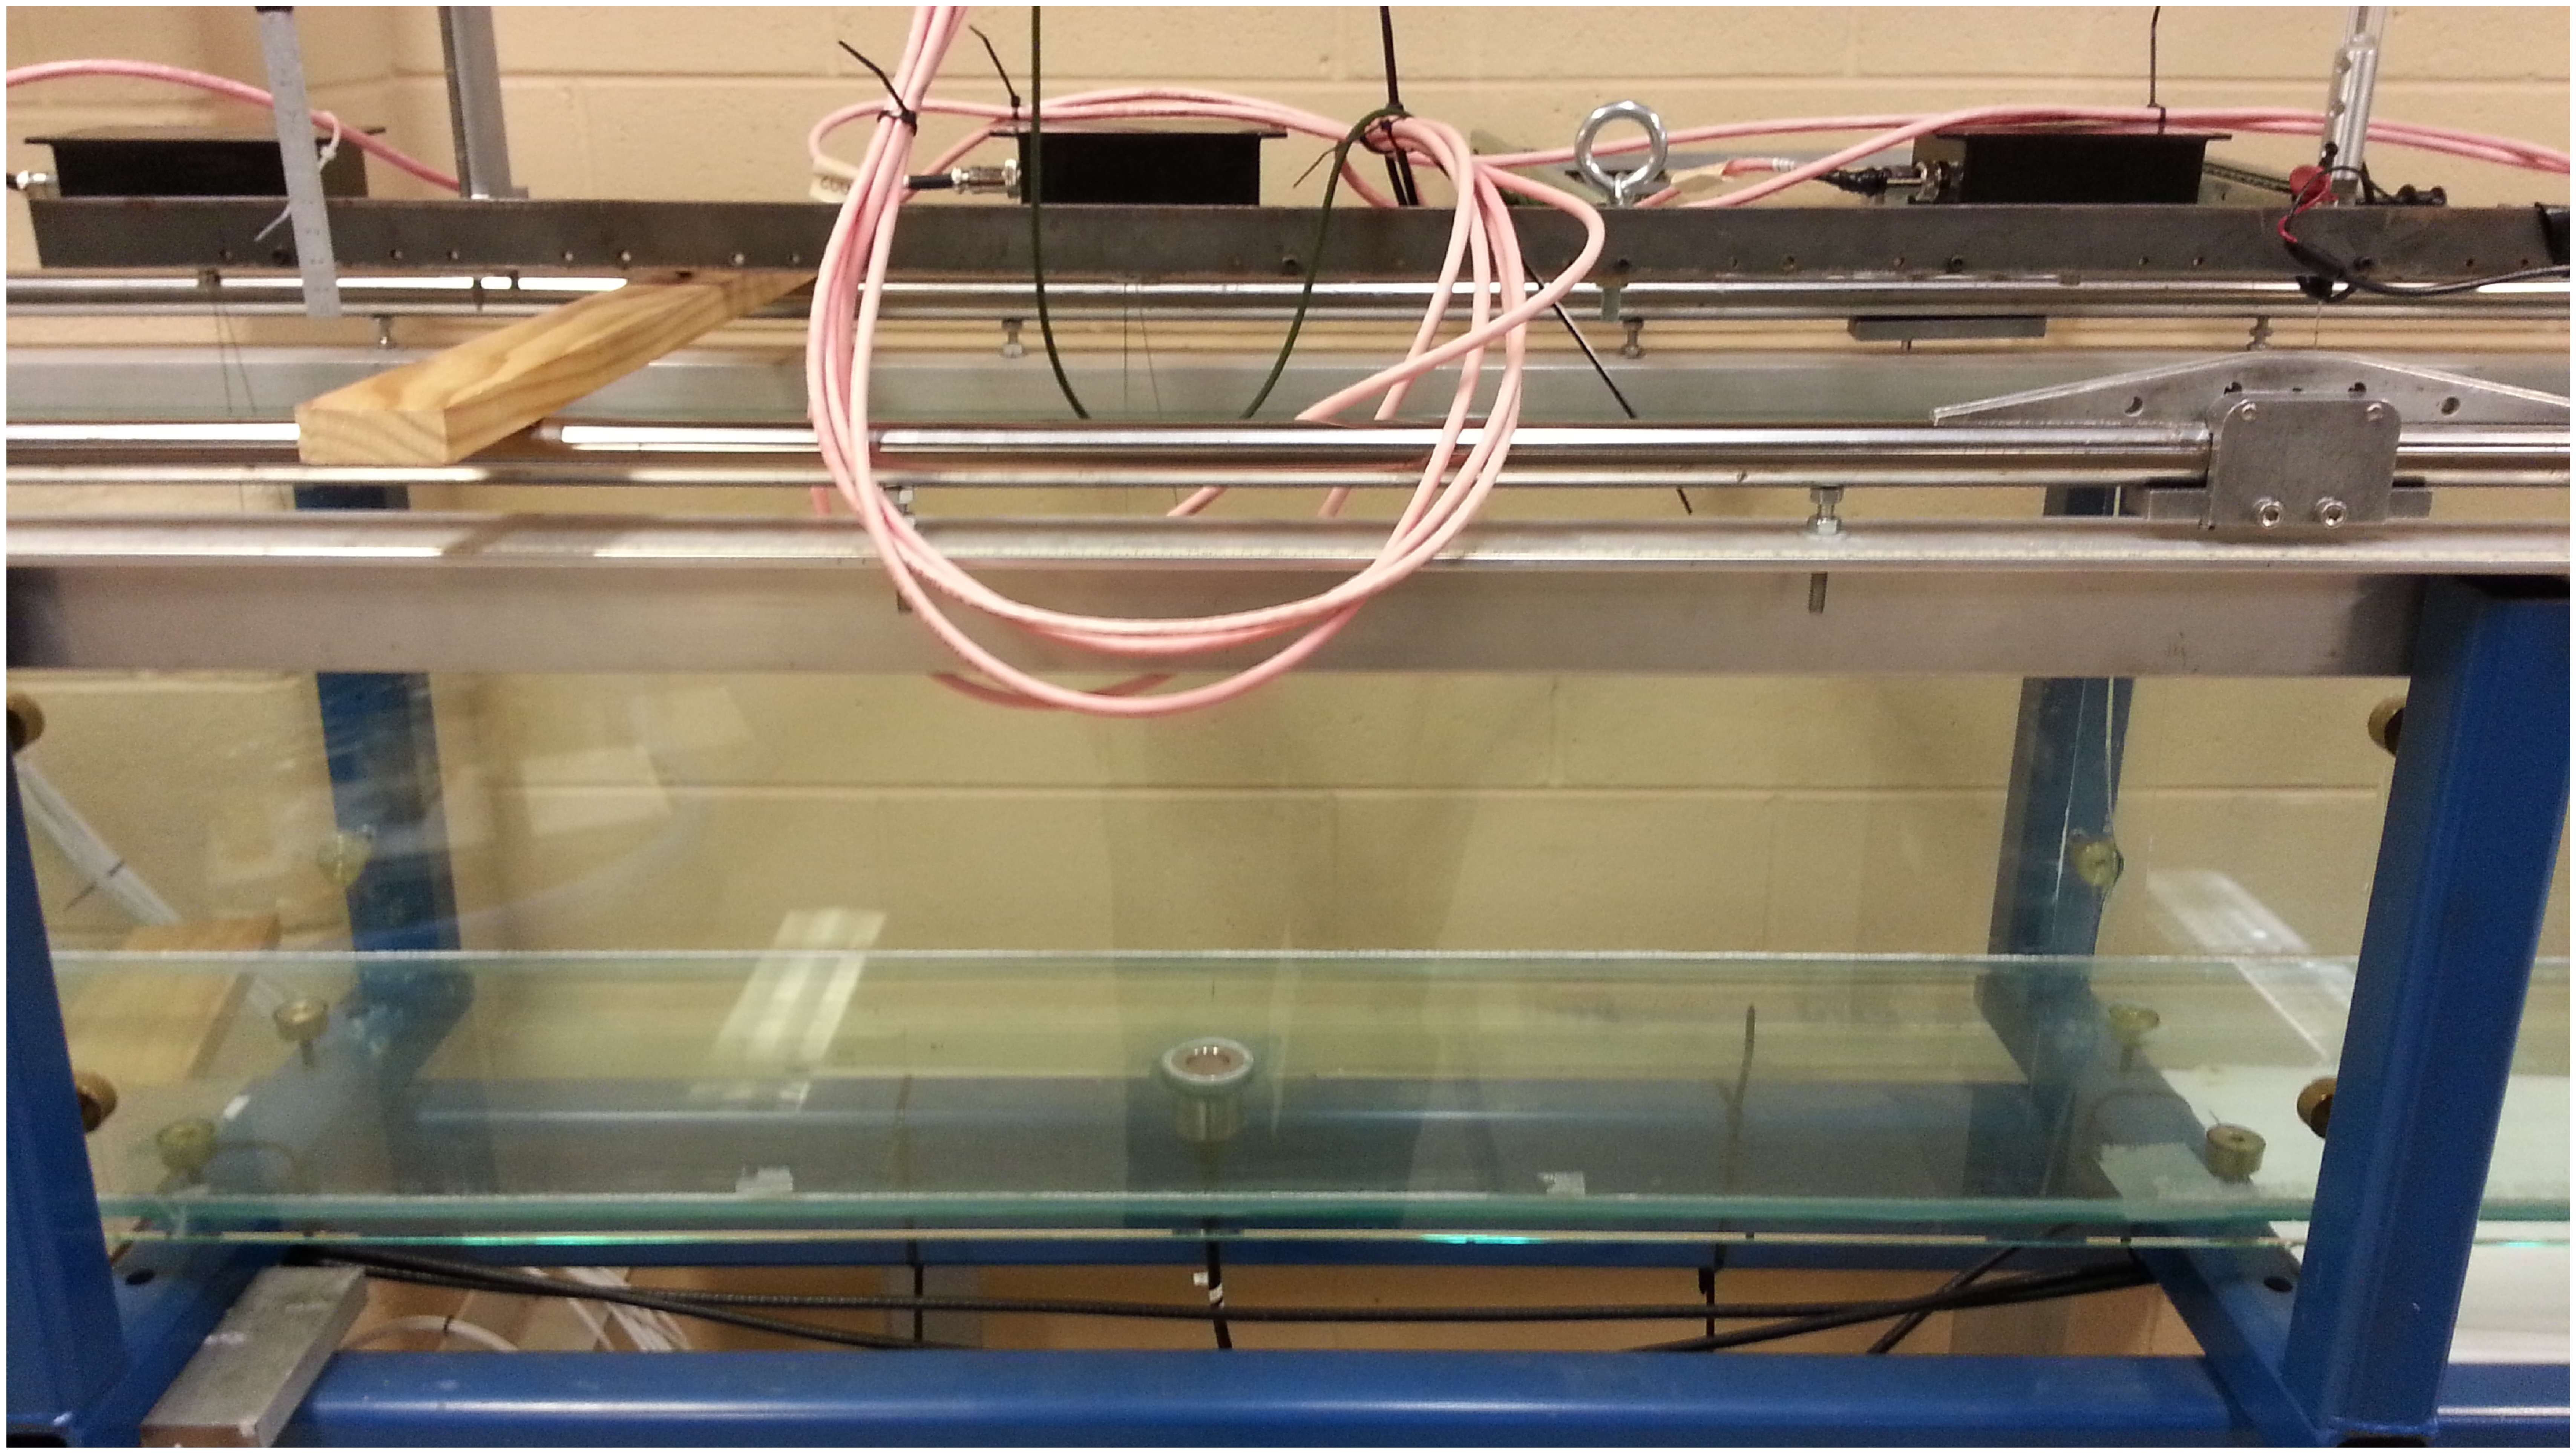
\includegraphics[height=.3\textheight]{images/Pressure_Sensor}
		\end{center}
	\vfill

}
% ==============================================================================================

\begin{frame}[t]
	\frametitle{}
		\begin{center}
		\vfill
		\only<1>{\Huge{\emB{Movie Time!}}}
		
		\vfill
		\end{center}
\end{frame}
% ==============================================================================================
% ==============================================================================================
\frame[t]{
	\frametitle{Experimental Set-Up}
	\vfill
	\begin{center}
		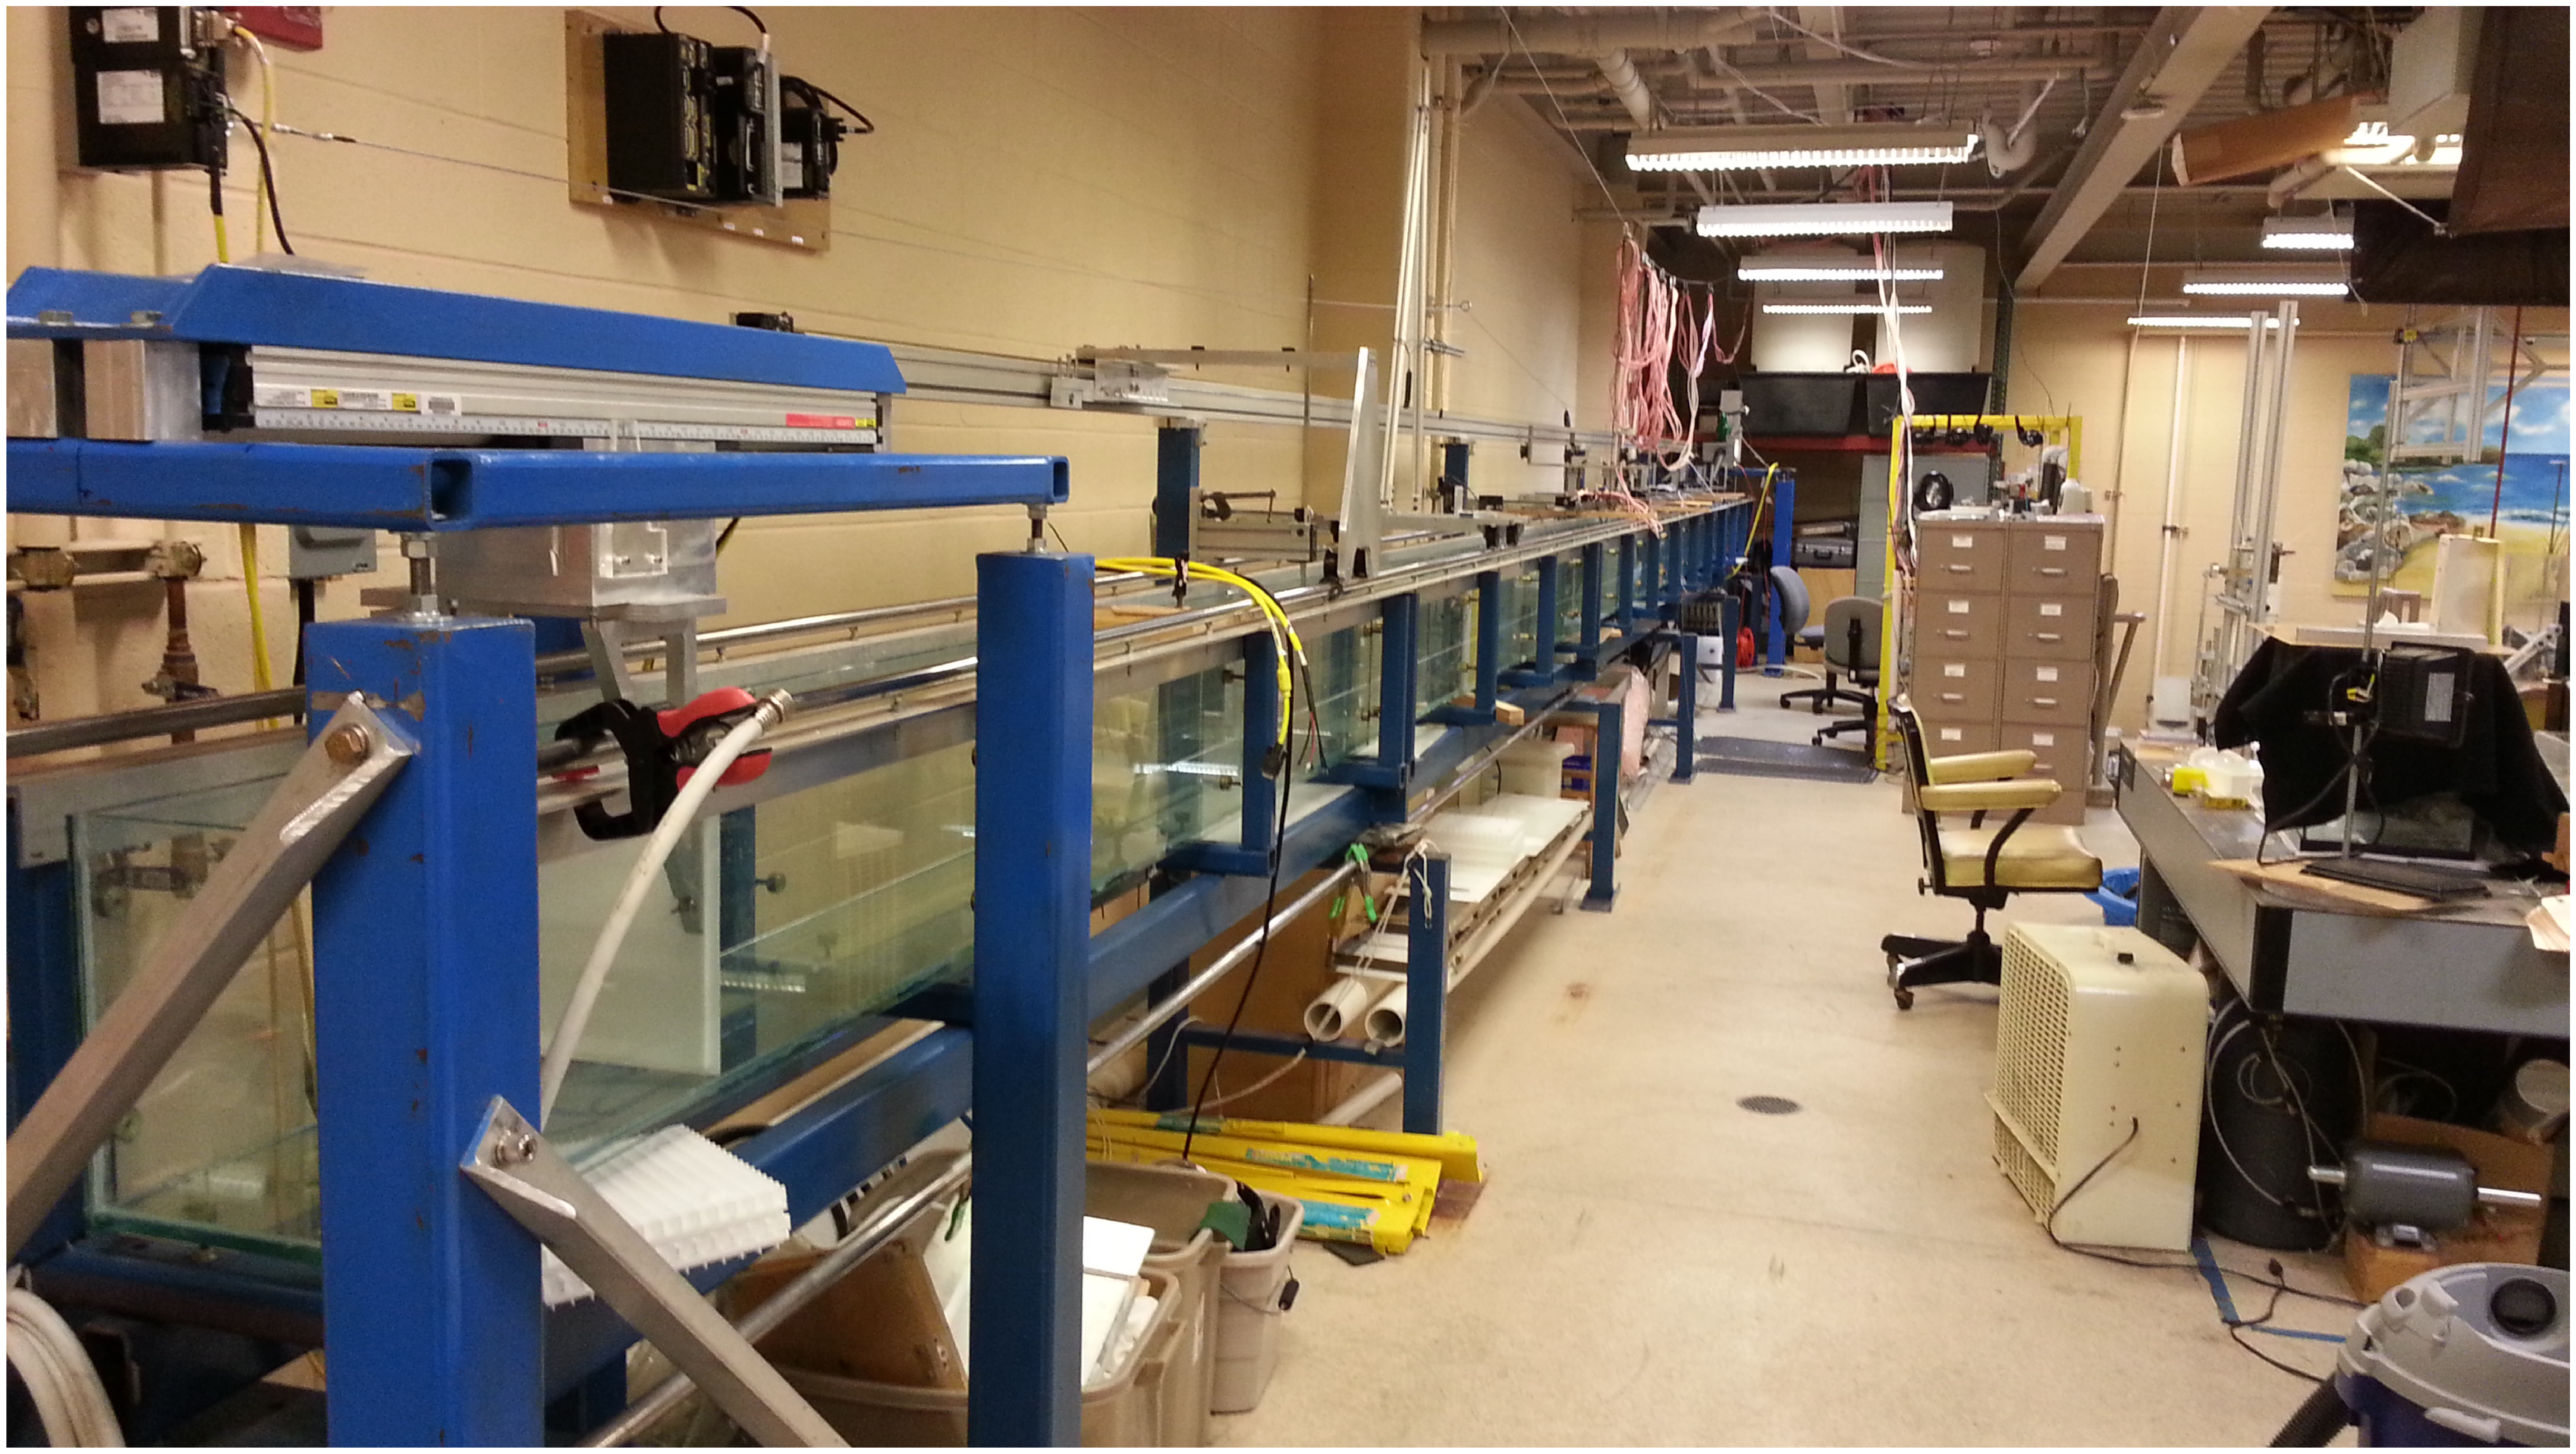
\includegraphics[height=.4\textheight]{images/Tank}
		\vfill
		\vfill
		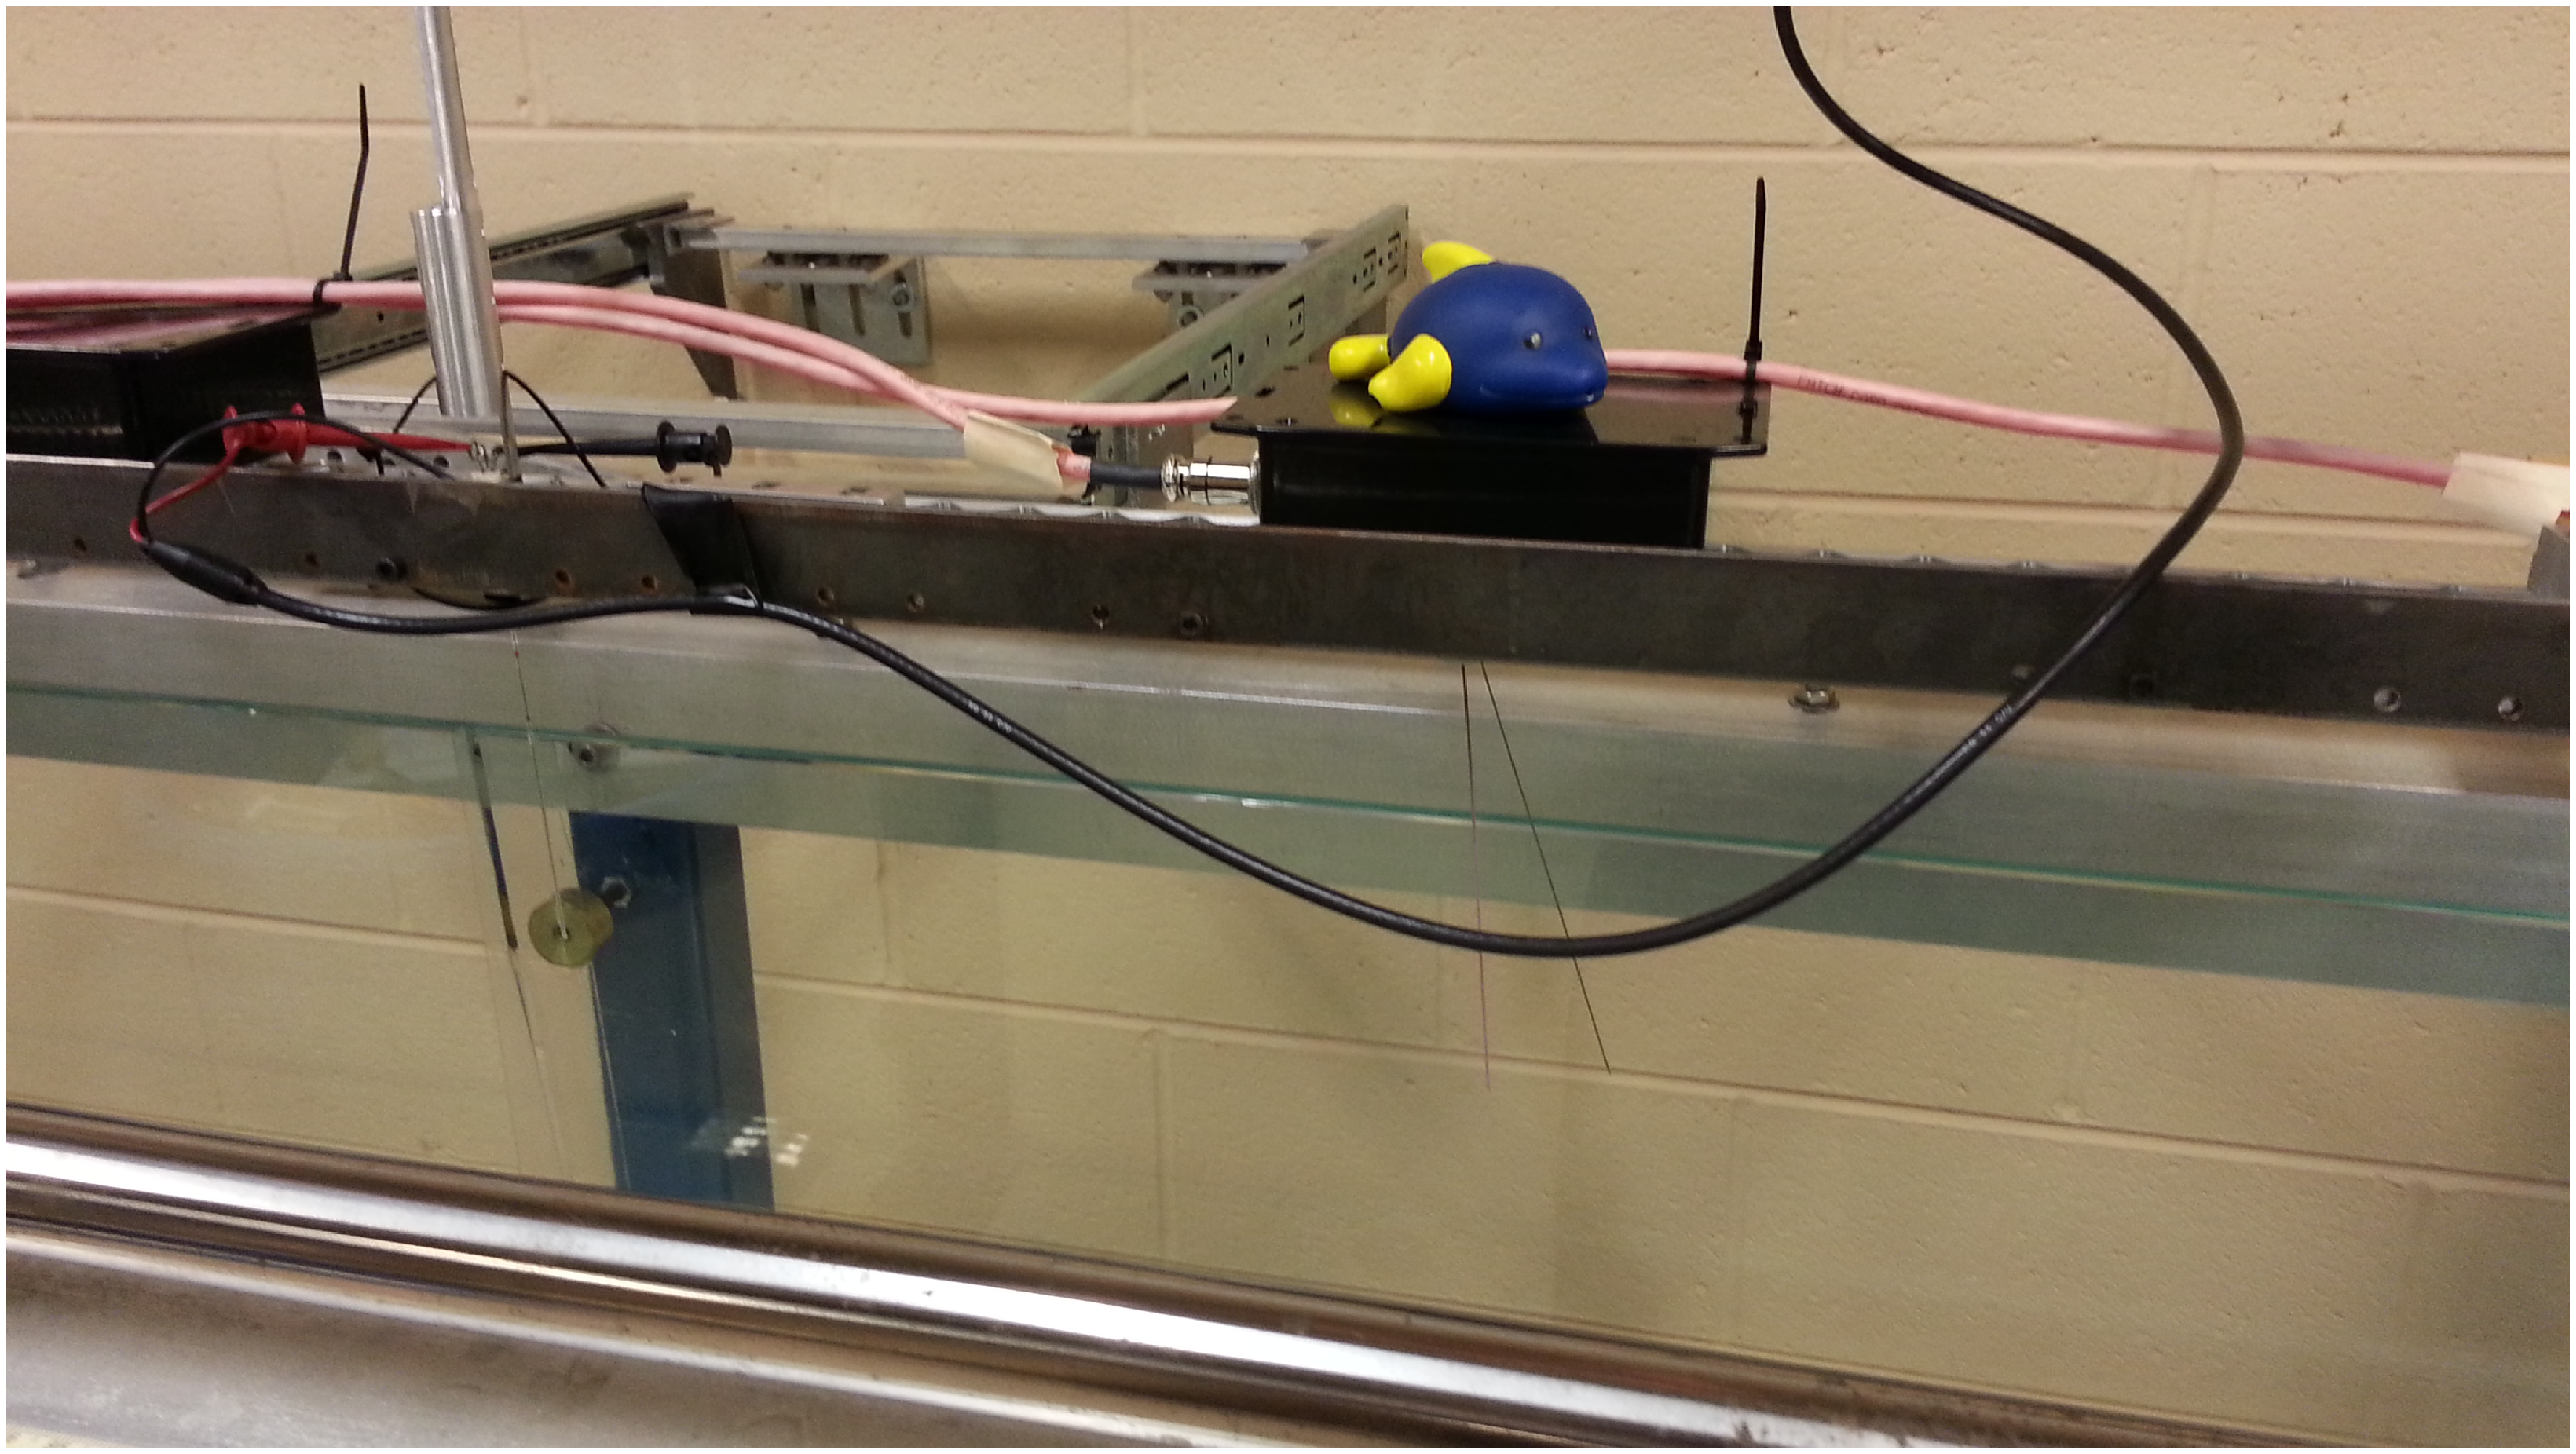
\includegraphics[height=.3\textheight]{images/Surface_Gauge}\hfill 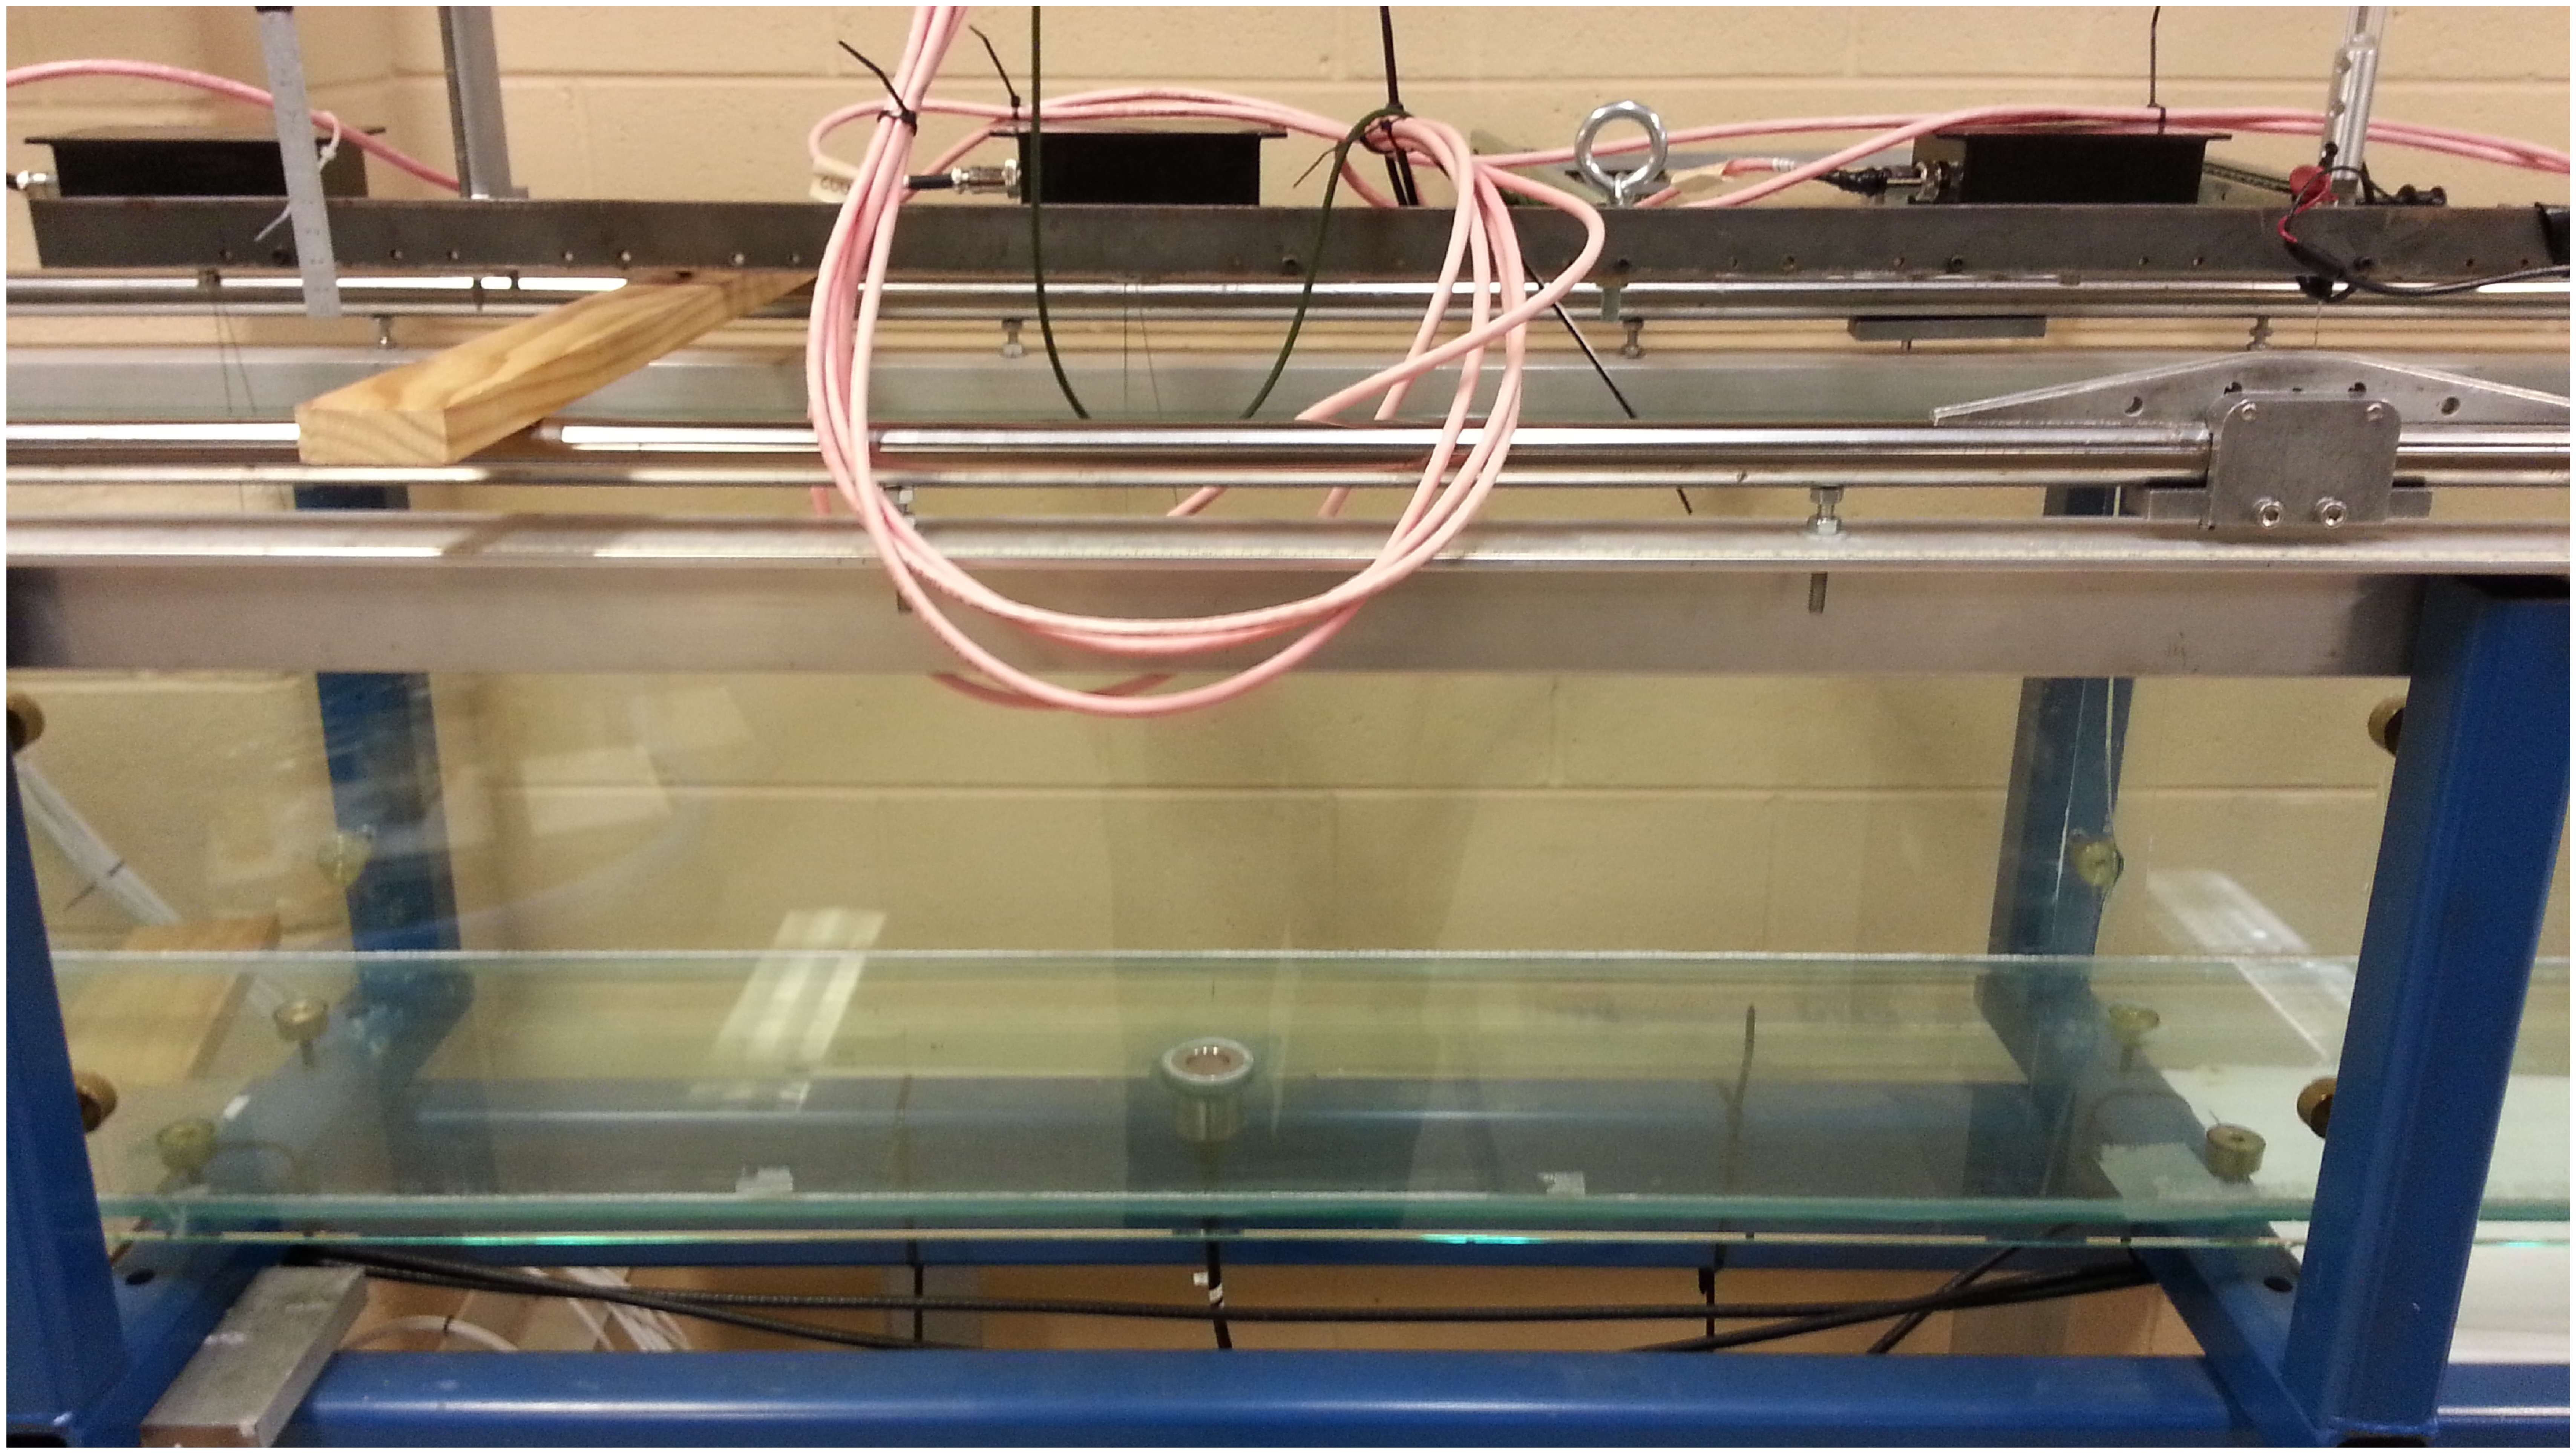
\includegraphics[height=.3\textheight]{images/Pressure_Sensor}
		\end{center}
	\vfill

}
% ==============================================================================================


% ==============================================================================================
\frame[t]{\frametitle{Experimental Data}
	\vfill
	\begin{figure}
		\centering
		{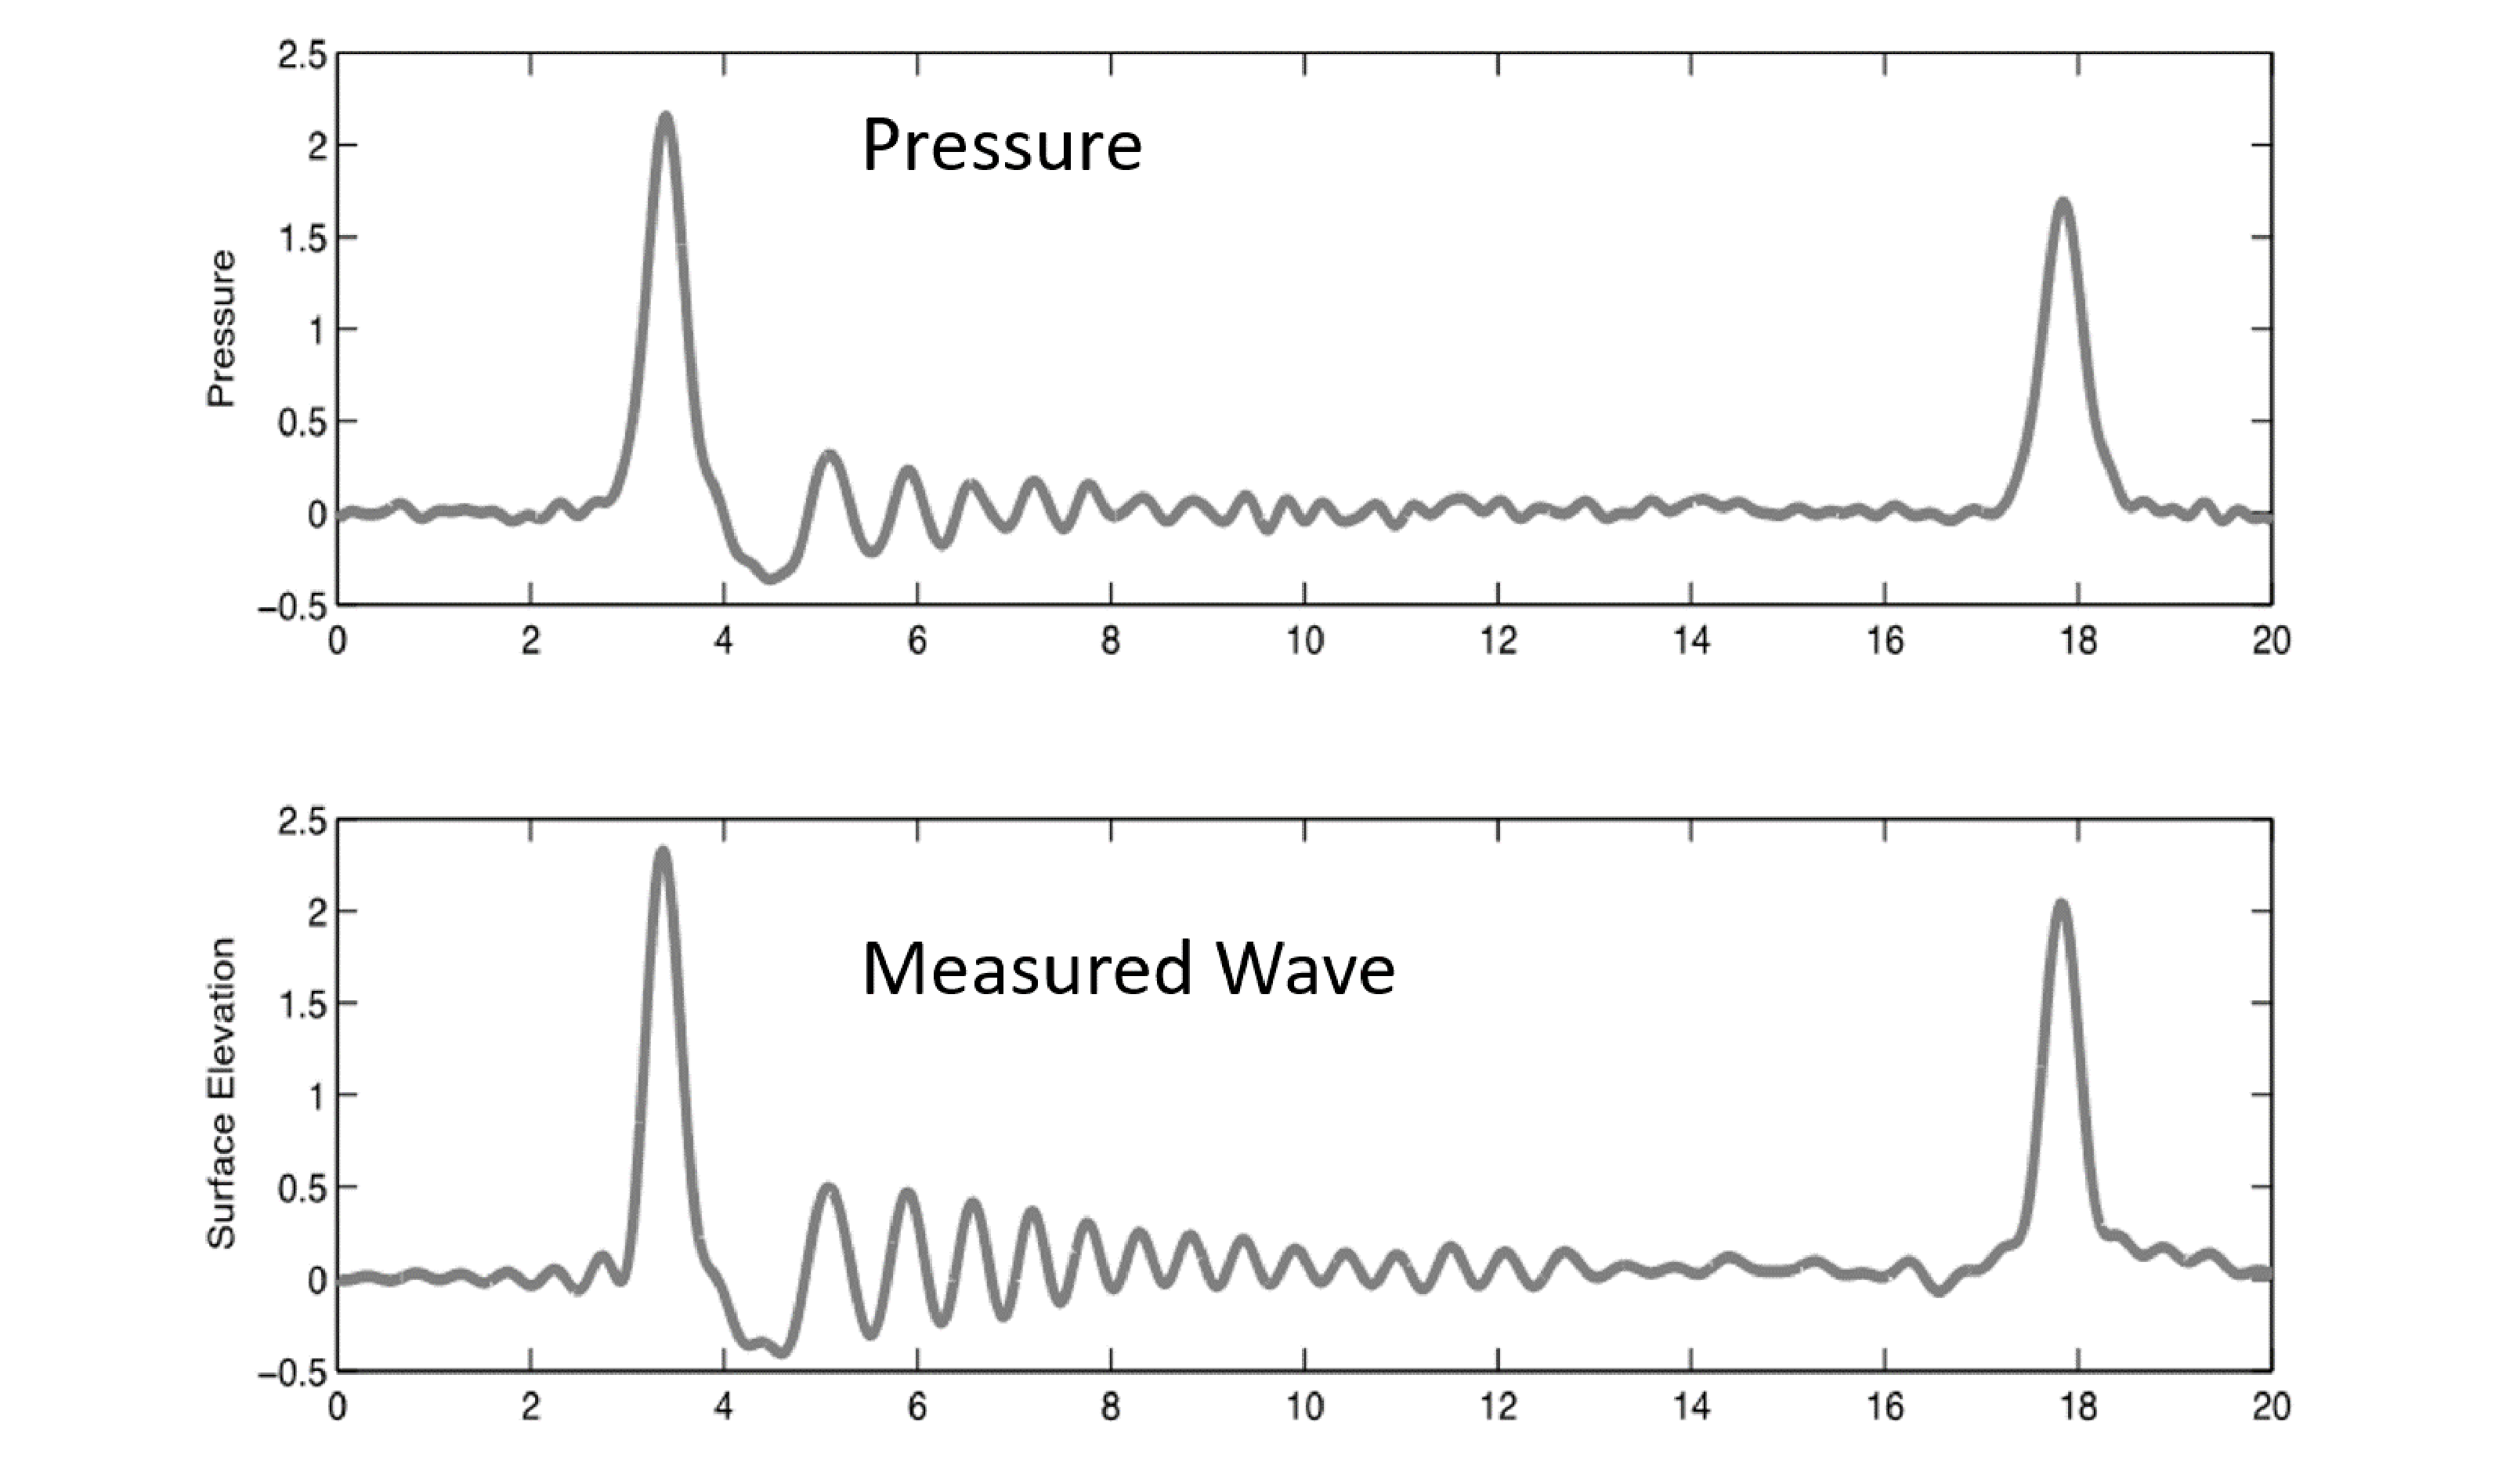
\includegraphics[width=.9\textwidth]{images/experimental_data}}%
		% \only<3>{\includegraphics[width=.9\textwidth]{images/experimental_data_b.png}}%
		% \only<2>{\includegraphics[width=.9\textwidth]{images/experimental_data_a.png}}%
		% \only<4>{\includegraphics[width=.9\textwidth]{images/experimental_data_c.png}}%
		% %\only<3>{\includegraphics[width=.95\textwidth]{images/experimental_data_d.png}}%
		% %\only<2>{\includegraphics[width=.95\textwidth]{images/experimental_data_e.png}}%
		% \caption{Time-series data converted to a spatial series using $c = \sqrt{g h}$.}
		\end{figure}
	\vfill
}
% ==============================================================================================

% ==============================================================================================
\begin{frame}[t]\frametitle{Experimental Results using \(\eta = P_d - \frac{h}{g}P_{d,tt}\)}
	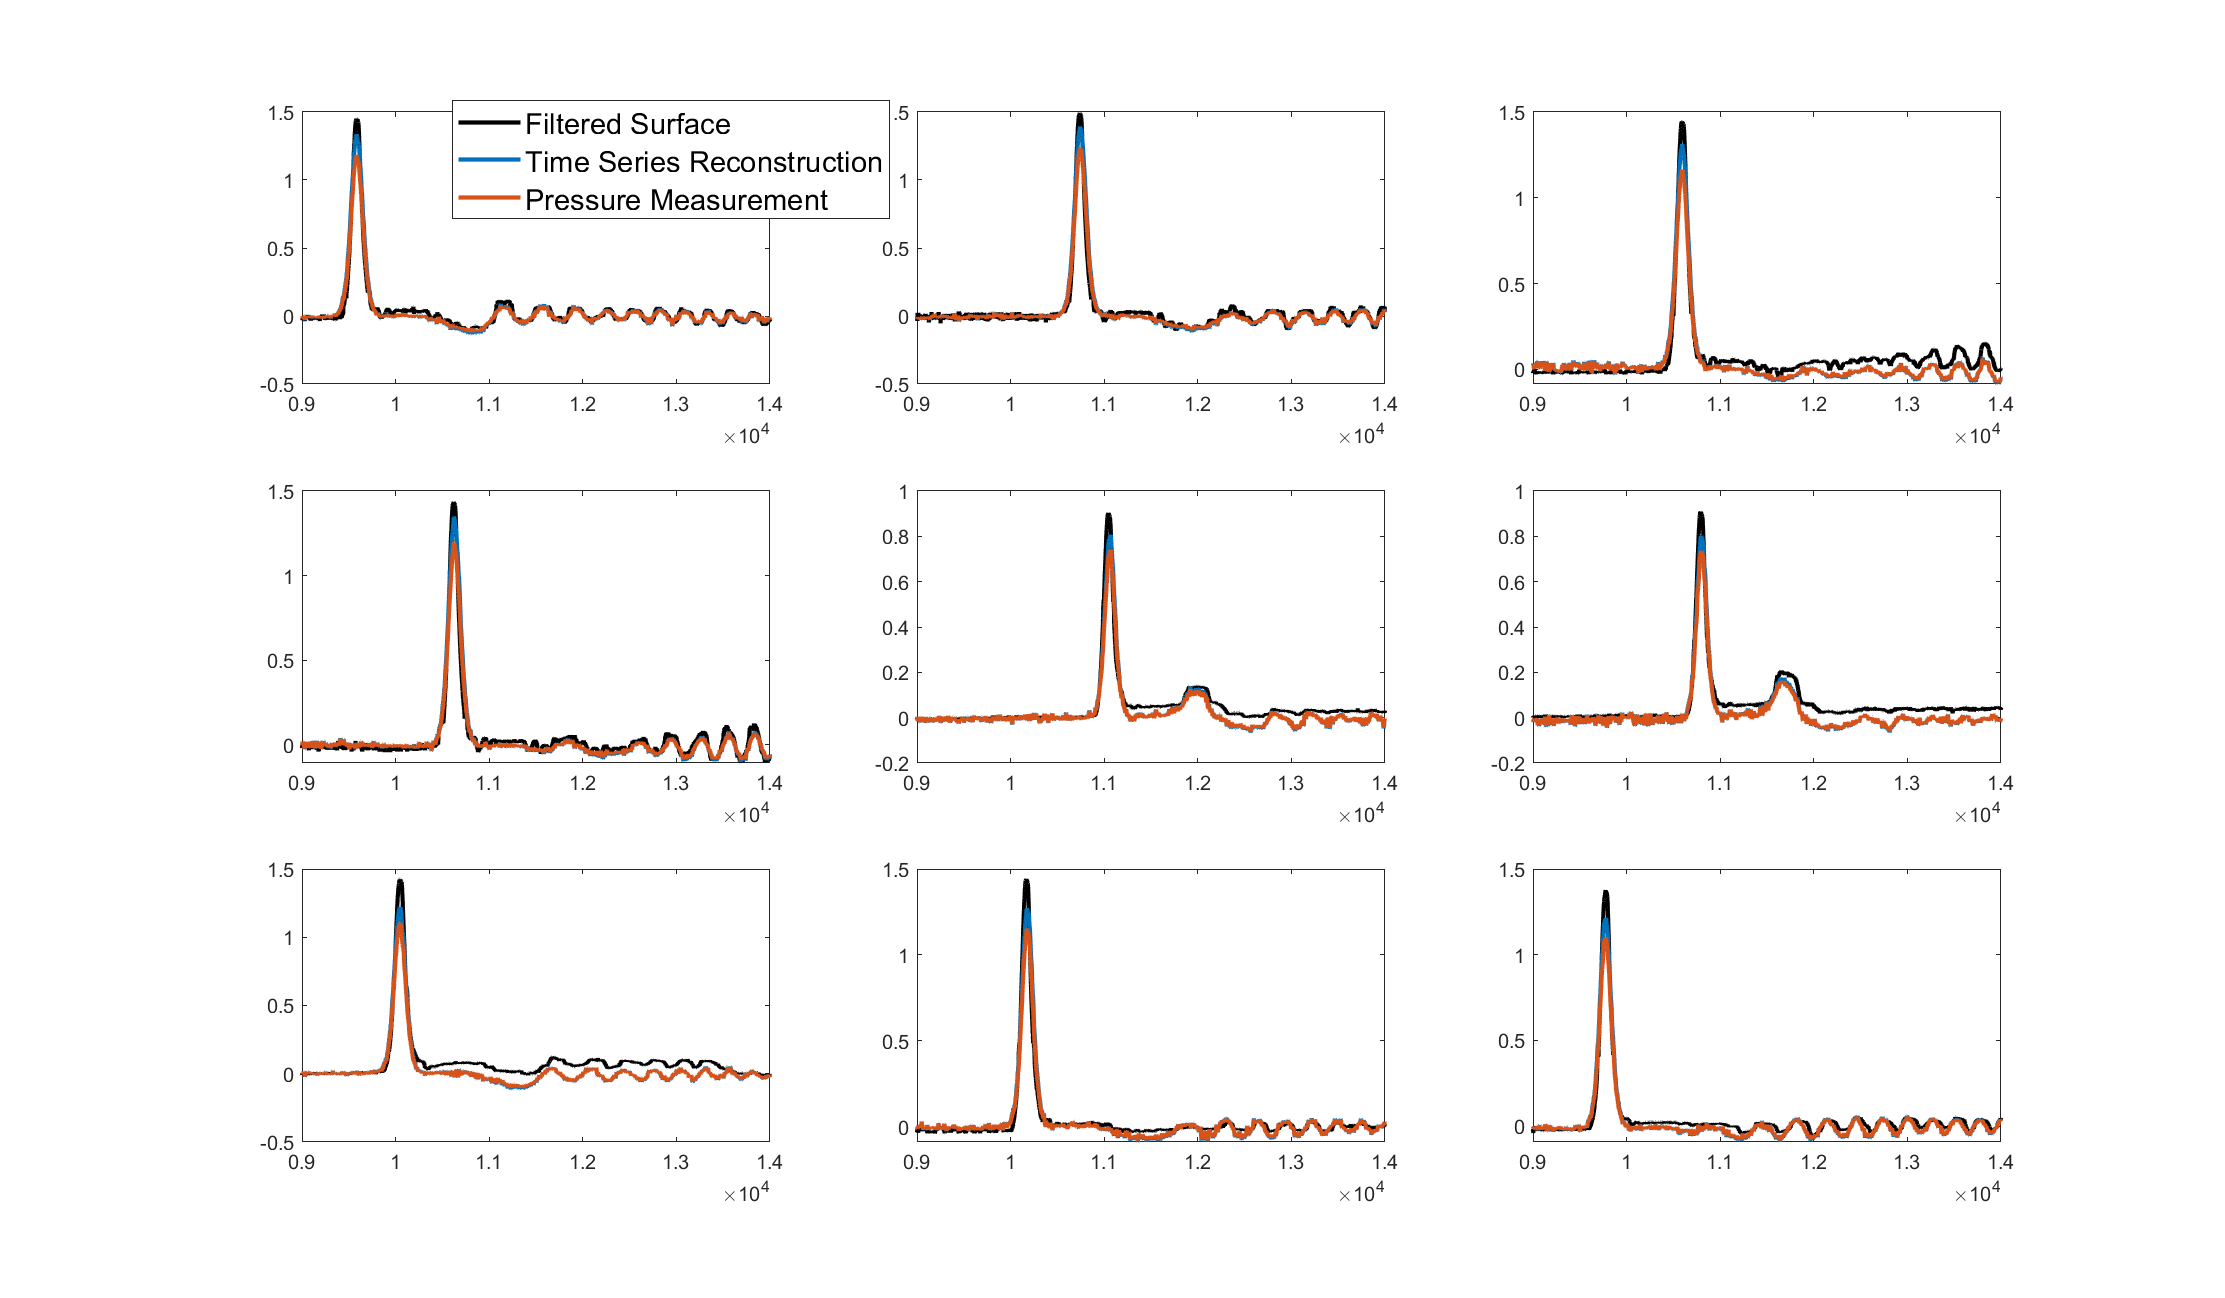
\includegraphics[height=.9\textheight]{images/nine_experiments_run.eps}
\end{frame}
% ==============================================================================================

% ==============================================================================================
\begin{frame}[t]\frametitle{Experimental Results using \(\eta = P_d - \frac{h}{g}P_{d,tt}\) with \(h = \) 5.05cm}
	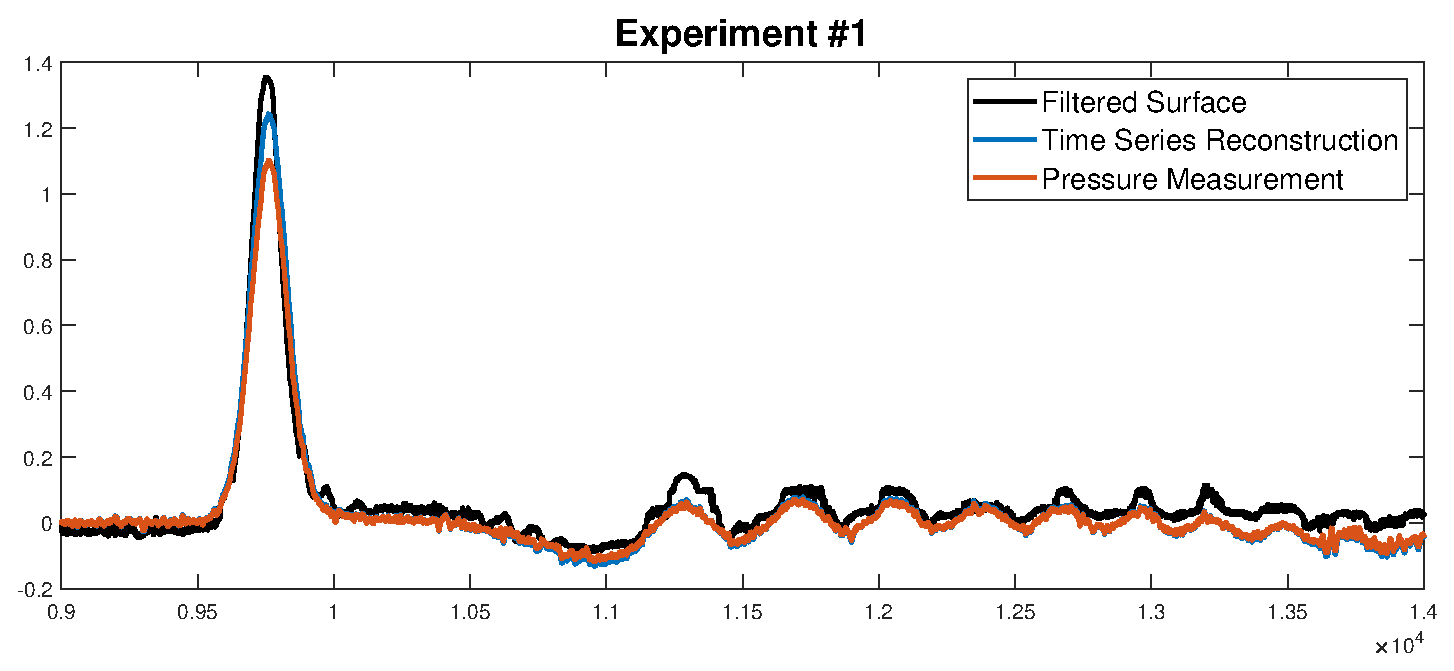
\includegraphics[width=\textwidth]{images/Exp_num_1.eps}
\end{frame}
% ==============================================================================================

% ==============================================================================================
\begin{frame}[t]\frametitle{Experimental Results using \(\eta = P_d - \frac{h}{g}P_{d,tt}\) with \(h = \) 5.05cm}
	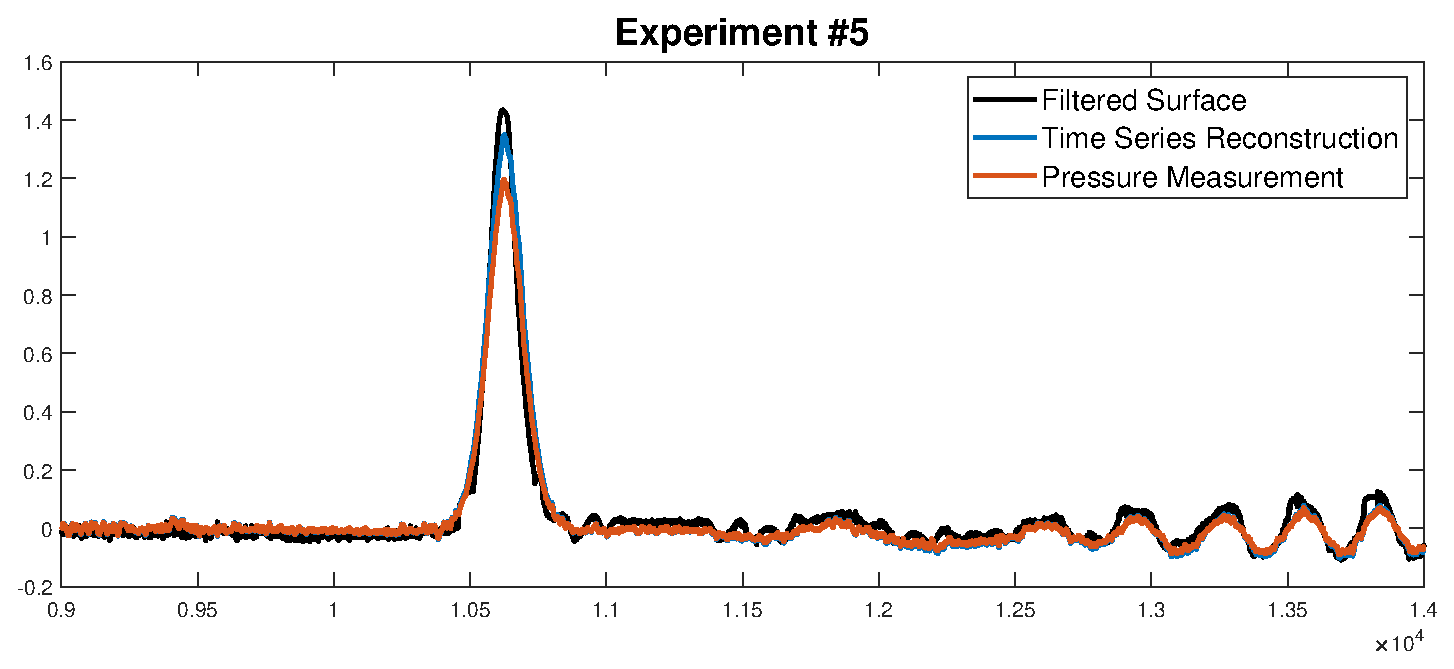
\includegraphics[width=\textwidth]{images/Exp_num_5.eps}
\end{frame}
% ==============================================================================================


% ==============================================================================================
\begin{frame}[t]\frametitle{Experimental Results using \(\eta = P_d - \frac{h}{g}P_{d,tt}\) with \(h = \) 3.55cm}
	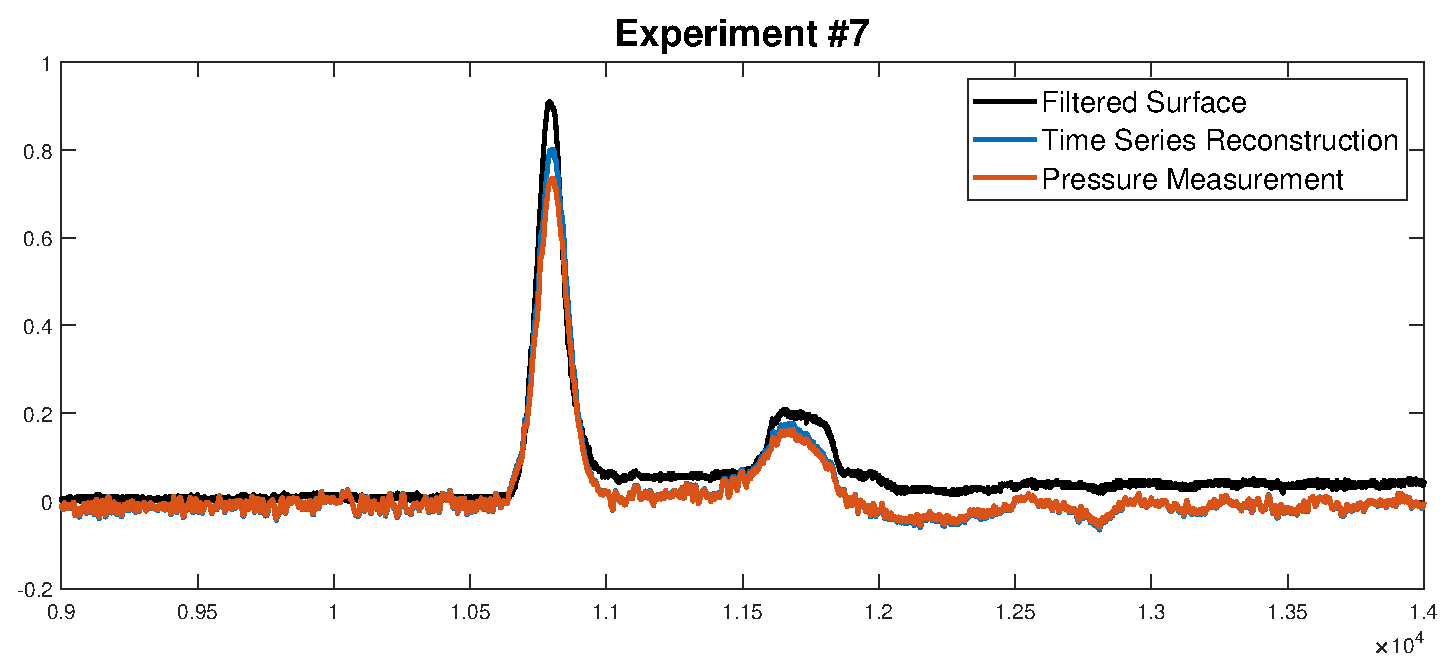
\includegraphics[width=\textwidth]{images/Exp_num_7.eps}
\end{frame}
% ==============================================================================================

% ==============================================================================================
\begin{frame}[t]\frametitle{Experimental Results using \(\eta = P_d - \frac{h}{g}P_{d,tt}\) with \(h = \) 4.10cm}
	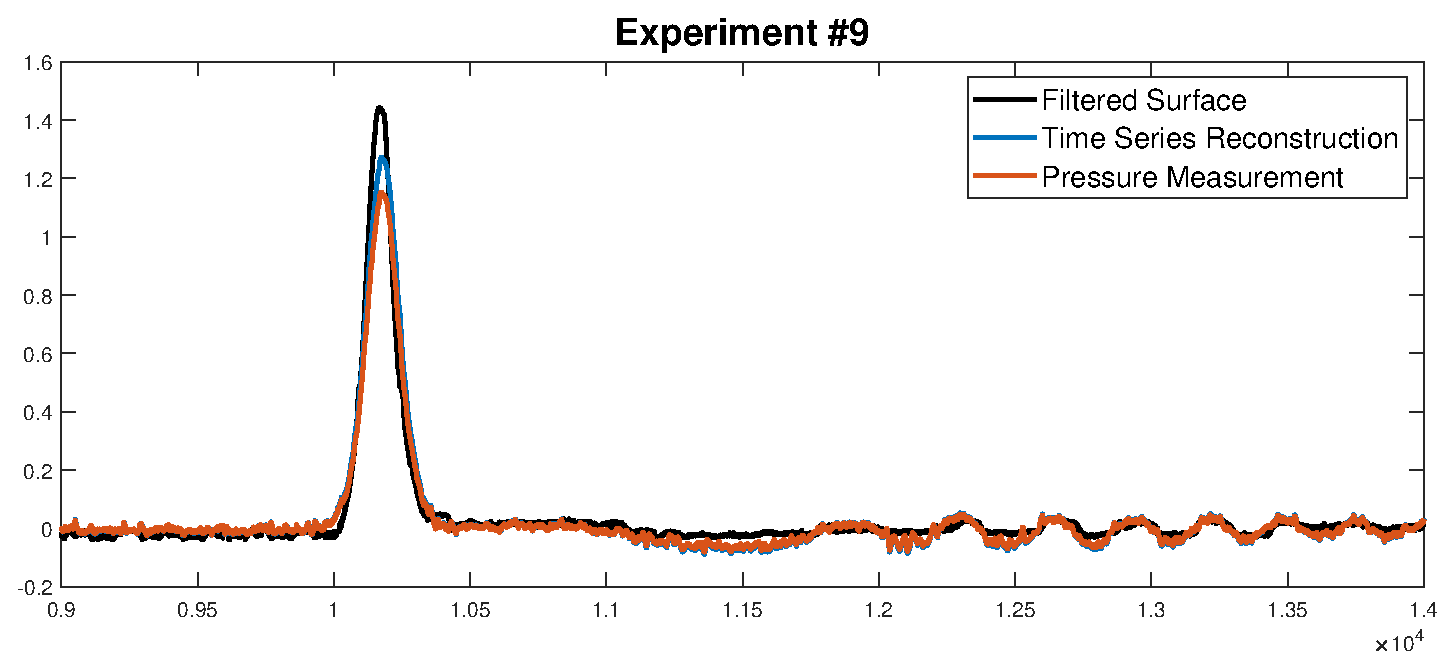
\includegraphics[width=\textwidth]{images/Exp_num_9.eps}
\end{frame}
% ==============================================================================================


